%; whizzy paragraph -pdf xpdf -latex ./whizzypdfptex.sh
%; whizzy-paragraph "^\\\\begin{frame}\\|\\\\emtext"
% latex beamer presentation.
% platex, latex-beamer でコンパイルすることを想定。 

%     Tokyo Debian Meeting resources
%     Copyright (C) 2012 Junichi Uekawa

%     This program is free software; you can redistribute it and/or modify
%     it under the terms of the GNU General Public License as published by
%     the Free Software Foundation; either version 2 of the License, or
%     (at your option) any later version.

%     This program is distributed in the hope that it will be useful,
%     but WITHOUT ANY WARRANTY; without even the implied warreanty of
%     MERCHANTABILITY or FITNESS FOR A PARTICULAR PURPOSE.  See the
%     GNU General Public License for more details.
%     You should have received a copy of the GNU General Public License
%     along with this program; if not, write to the Free Software
%     Foundation, Inc., 51 Franklin St, Fifth Floor, Boston, MA  02110-1301 USA

\documentclass[cjk,dvipdfmx,12pt]{beamer}
\usetheme{Tokyo}
\usepackage{monthlypresentation}

%  preview (shell-command (concat "evince " (replace-regexp-in-string "tex$" "pdf"(buffer-file-name)) "&")) 
%  presentation (shell-command (concat "xpdf -fullscreen " (replace-regexp-in-string "tex$" "pdf"(buffer-file-name)) "&"))
%  presentation (shell-command (concat "evince " (replace-regexp-in-string "tex$" "pdf"(buffer-file-name)) "&"))

%http://www.naney.org/diki/dk/hyperref.html
%日本語EUC系環境の時
\AtBeginDvi{\special{pdf:tounicode EUC-UCS2}}
%シフトJIS系環境の時
%\AtBeginDvi{\special{pdf:tounicode 90ms-RKSJ-UCS2}}

\newenvironment{commandlinesmall}%
{\VerbatimEnvironment
  \begin{Sbox}\begin{minipage}{1.0\hsize}\begin{fontsize}{8}{8} \begin{BVerbatim}}%
{\end{BVerbatim}\end{fontsize}\end{minipage}\end{Sbox}
  \setlength{\fboxsep}{8pt}
% start on a new paragraph

\vspace{6pt}% skip before
\fcolorbox{dancerdarkblue}{dancerlightblue}{\TheSbox}

\vspace{6pt}% skip after
}
%end of commandlinesmall

\title{初めてのキーサインパーティ}
\author{齋藤 雄介  ysaito@golangcoder.club}
\date{2017年9月16日}
\logo{
\includegraphics[width=8cm]{image200607/openlogo-light.eps}}

\begin{document}

\begin{frame}
\titlepage{}
\end{frame}

\begin{frame}{参考にした資料}
  キーサインパーティで参考にさせていただいた資料

  %%BoundingBox: 0.00 0.00 362.83 272.13
  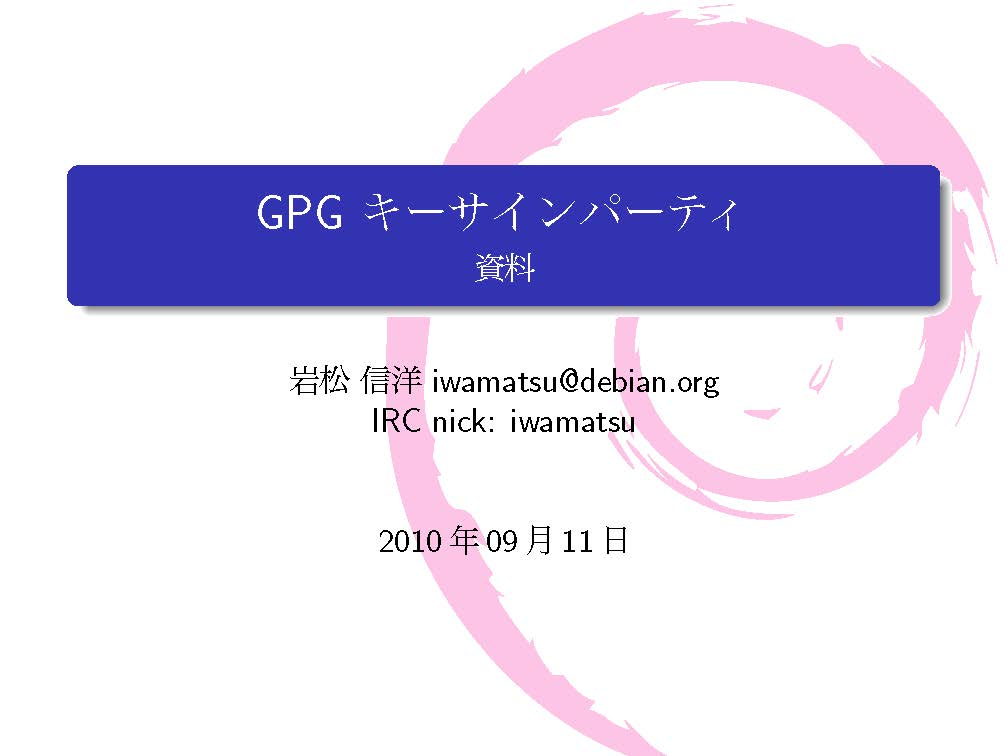
\includegraphics[width=0.8\hsize]{image201709/shiryo001.jpg}
  \end{frame}


\section{}
%\emtext{}

\begin{frame}[containsverbatim]{caffを使おうとして}
Homebrew から消えてた
\begin{commandline}
$ brew search signing-party
 ==> Searching local taps...
 ==> Searching taps on GitHub...
 ==> Searching blacklisted, migrated and deleted formulae...
 signing-party was deleted from homebrew/core in commit e05298ad8a:
\end{commandline}
\end{frame}

\begin{frame}{gpgのみでやってみよう}
  %%BoundingBox: 0.00 0.00 362.83 272.13
  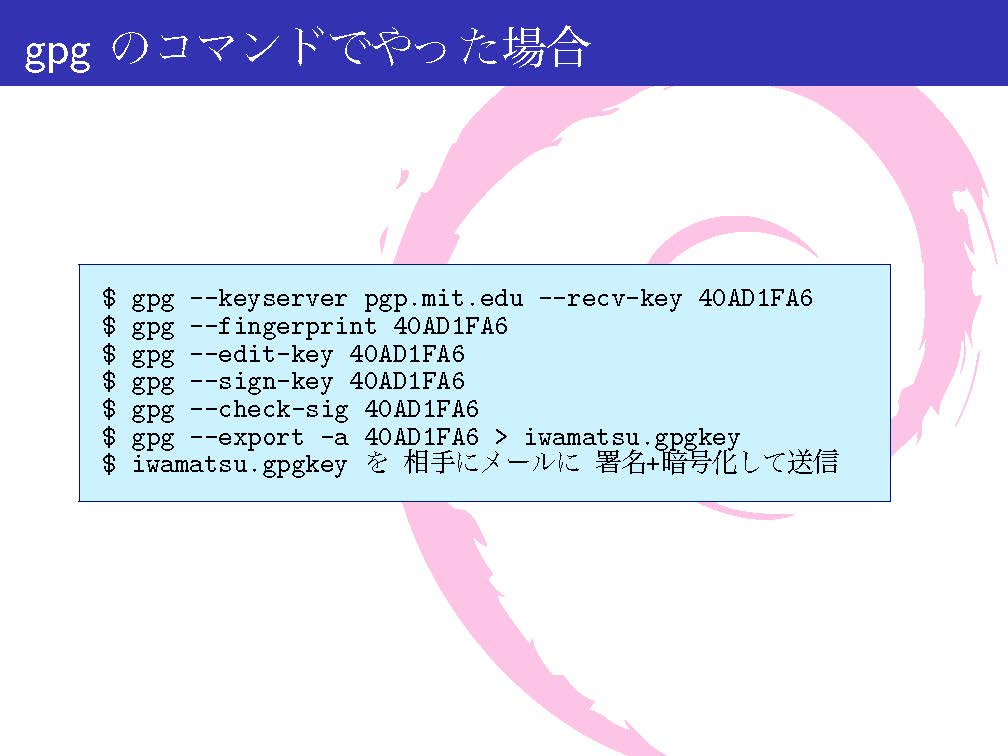
\includegraphics[width=0.8\hsize]{image201709/shiryo002.jpg}
\end{frame}

\begin{frame}[fragile]{つまづいた}
相手の公開鍵で暗号化するところを自分の公開鍵で暗号化してしまった
\begin{commandline}
$ gpg --encrypt --recipient 相手の公開鍵ID 相手の公開鍵
\end{commandline}
  %%BoundingBox: 0.00 0.00 362.83 272.13
  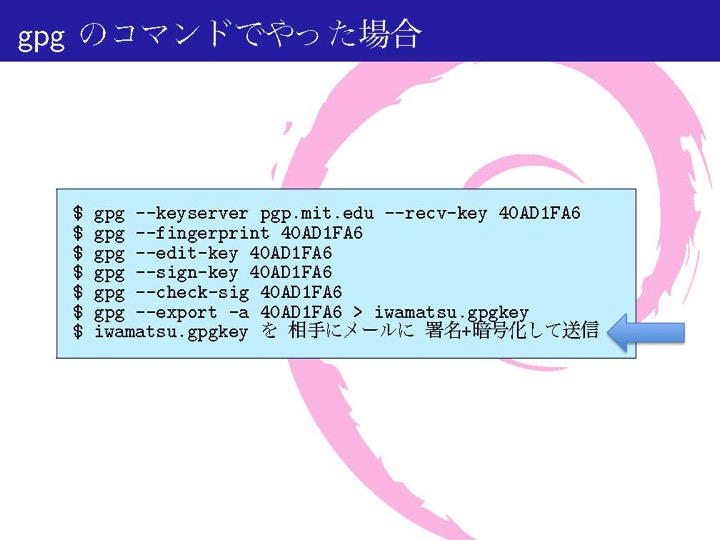
\includegraphics[width=0.8\hsize]{image201709/shiryo003.jpg}
\end{frame}

\begin{frame}[containsverbatim]{caffをつかわないなら}
参考: https://github.com/thinkAmi/caffish-ps
\begin{commandline}
# キーサーバより相手の公開鍵を取得し、
# 自分の公開鍵の鍵束に入れる
$ gpg --keyserver pgp.mit.edu --recv-key 相手の公開鍵ID

# 表示されるフィンガープリントと、
# 手元の書類のフィンガープリントが一致していることを確認
$ gpg --fingerprint 相手の公開鍵ID

# 相手の公開鍵に署名
$ gpg --sign-key 相手の公開鍵ID

# 署名した公開鍵をエクスポート
$ gpg --export -a 相手の公開鍵ID > ./foo.gpgkey

# 自分の秘密鍵で署名した相手の公開鍵を、相手の公開鍵を使って暗号化
$ gpg --no-auto-check-trustdb  --trust-model=always \
  --armor --recipient 相手の公開鍵ID --encrypt ./foo.gpgkey
# foo.gpgkey.asc が生成される
# 暗号化した公開鍵をメールに添付し、
# メール本文を暗号化して相手へ送信
\end{commandline}
\end{frame}

\begin{frame}
\Huge そうだ caff つかおう 
\end{frame}

\begin{frame}[fragile]{もう一つ詰まったところ}
  Debian strech に caff をいれて
  メールサーバを立てて...
  \begin{commandline}
$ caff -u 自分の公開鍵ID 一人目の公開鍵ID 二人目の公開鍵ID...
[NOTICE] Fetching keys from pool.sks-keyservers.net, this may take a while...
[WARN] Local-user 自分の公開鍵ID is not defined as one of your keyid in ~/.caffrc (it will not be used)
[ERROR] None of the local-user keys seem to be known as a keyid listed in ~/.caffrc
# ~/.caffrc はちゃんと設定しているはずだけど...
# 自分の公開鍵のフィンガープリントの後半16桁

$ caff 一人目の公開鍵ID 二人目の公開鍵ID...
# 通った
  \end{commandline}
  
\end{frame}

\end{document}

;;; Local Variables: ***
;;; outline-regexp: "\\([ 	]*\\\\\\(documentstyle\\|documentclass\\|emtext\\|section\\|begin{frame}\\)\\*?[ 	]*[[{]\\|[]+\\)" ***
;;; End: ***

